\chapter{Implementation}
\label{implementation}
We present a computer program which takes in a textual phrase in English, determines all oronyms for that phrase, and then visualizes those oronyms in two ways: tree form, with branch width scaled by word frequency metrics to indicate the likelihood of interpretation; and in sunburst diagram form, where all valid oronyms radiate from a center root, with each arc scaled by frequency.

To accomplish this, the program has four major functional parts: a custom phonetic dictionary, a command-line oronym generator, an OpenGL oronym-parse-tree visualization generator, and a Protovis datafile generator. 

\section{Customized Phonetic Dictionary} 
\label{section:Implementation:customizedPhoneticDictionary}

In order to discover oronyms for each phrase, we first needed to determine how each phrase is pronounced.  Pronunciation can vary depending on the speaker's accent, so it was important for us to (1) chose an accent that we could easily replicate and (2) find a dictionary that supported that accent.  

\subsection{Accent Choice}
We decided to utilize a General American accent, due to its ubiquity in media and news sources. The General American accent, also known as the ``Standard American English" dialect, is not spoken by most Americans, but is used as an ``average accent".  It most closely resembles the Midwestern accent used in the area in Figure~\ref{fig:generalAmericanMap}, but is more commonly recognized as ``the newscaster accent". Newscasters learn this accent for use on national TV, because it is the ``least-accented" of the American accents\cite{JaneBarbe}.  

\begin{center}
\begin{figure}
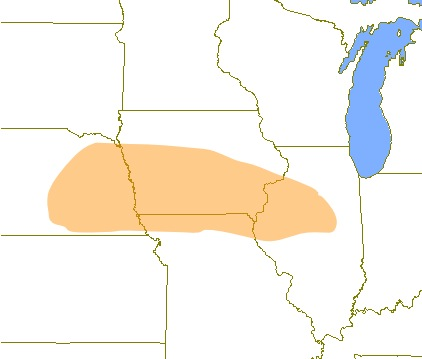
\includegraphics[width=60mm]{General_American.jpg}
\captionfonts
\caption[Geographic Origin of General American]{This is the geographic area whose accent most closely resembles the General American Accent \cite{generalAmericanAccentMap} }
\label{fig:generalAmericanMap}
\end{figure}
\end{center}
The downside of using the General American accent is that, while it does give a good approximation of most American's speaking accents, it does not perfectly reflect a ``singing accent''. Singers tend to elongate syllables, changing emphasis placement in words, and vowels tend to be sung in a more ``round'' matter\cite{onSingingAccentsDCblog}.For example, though the dictionary pronunciation of the word ``baby'' is \texttt{"be\$bi} (bay-bee), in songs, you commonly hear the pronunciation \texttt{"be\$be} (bay-bay). The \texttt{e} sound is easier to sing than the \texttt{i} (ee) sound, because the latter requires the singer move their mouth and vocal cord position further from neutral than the former does\cite{technicalDescriptionOfVowelSinging}.

However, since different singers will change pronunication for different vowels based upon which vowels are easiest for them to sing, no definitive pronunciation guidelines or rules exist. Therefore, using the General American accent gave us as good an approximation as we were likely to get\cite{whyAmericanEnglishIsNoAccent}.

\subsection{Dictionary Options}
\label{subsection:dictionaryOptions}

We considered using three different phonetic dictionaries: the CMU dictionary, LC-STAR dictionary and UNISYN dictionary\cite{lcStarWebsite} \cite{cmuDictWebsite}  \cite{unisynLexiconWebsite}.  We started out by looking at the LC-STAR dictionary, but quickly decided that it wasn’t going to be as useful to us, because the LC-STAR dictionary is not particularly well-maintained.  

The CMU dictionary showed promise, but had a few shortcomings.  In its favor, it had a very simple way of encoding words:  first the orthographic word, then the identifier number in parentheses (if needed), then a space, then a one-to-two char code for each sound in the word, with the numbers 0, 1, 2 appended to indicate emphasis (if needed), separated by spaces.  An example of a CMU dictionary entry can be seen in Figure ~\ref{fig:CMUdictAbbreviate}.

\begin{figure}
\begin{center}
\begin{verbatim}
ABBREVIATE  AH0 B R IY1 V IY0 EY2 T
\end{verbatim}
\captionfonts
\caption[CMU dictionary entry example]{Here is the CMU dictionary entry for the word ``abbreviate" }
\label{fig:CMUdictAbbreviate}
\end{center}
\end{figure}




The problem that arose with this format, was that there was no explicit definition of where to hyphenate the word when splitting it up.  This causes problems for words in song lyrics, where each note has its own syllable underneath it, and each syllable might have many different sounds. In addition, it used non-standard symbols for its phonetic alphabet, which would complicate matters if, in the future, we chose to combine data from other dictionaries with our existing dictionary. Most importantly, the phonetic sequences, if the spaces were removed, would not be deterministically parsible. 

The UNISYN dictionary is used primarily to phonetically translate words into multiple accents.  It has its own formated dictionary, with a bunch of wildcards representing different phones.  UNISYN provides some semi-functioning perl scripts that allow you to specify a dialect you’d like to use (For example, a Californian would say ``cooking" differently than someone from the Deep South, and both would say it differently than someone from London.  However, they are all speaking English.  The UNISYN dictionary facilitates this translation).  

It had all the information we needed, and then some.  However, it was case-insensitve, meaning that it didn't make it easy to differenciate pronunciations for some words. For example, the word ``nice" is pronounced differently from the city ``Nice", but they were both stored as ``nice" in the orthography of UNISYN. This was a minor setback, but we were able to design our user study around this limitation, and ultimately decided to use the UNISYN dictionary exclusively.


\subsection{Custom dictionary fields}
\label{subsection:customDictionaryFields}

Below we lay out the format for the fields in an entry of our custom phonetic dictionary, which we generated using the UNISYN dictionary's perl script output for the General American accent:
\textcolor{Aquamarine}{$<$\textbf{ortho}$>$} :
\textcolor{BurntOrange}{$<$\textbf{uniqueID}$>$} :
\textcolor{RoyalBlue}{$<$\textbf{partOfSpeech}$>$} :
\textcolor{Red}{$<$\textbf{SAMPAspelling}$>$} :
\textcolor{Rhodamine}{$<$\textbf{SAMPAnoEmph}$>$} :
\textcolor{Periwinkle}{$<$\textbf{extendedOrtho}$>$} :
\textcolor{Blue}{$<$\textbf{freq}$>$}
\end{center}

\begin{figure}
Example:
\begin{center}
{\tt 
\textcolor{Aquamarine}{transfer} :
\textcolor{BurntOrange}{2} :
\textcolor{RoyalBlue}{VB/VBP} :
\textcolor{Red}{tr\{ns"f3`r} :
\textcolor{Rhodamine}{tr\{nsf3`r} :
\textcolor{Periwinkle}{\{trans==fer\}} :
\textcolor{Blue}{7184}
}
\captionfonts
\caption[Custom dictionary entry example]{Here is an example an entry in our custom phonetic dictionary, using the word ``transfer" }
\label{fig:customDictionaryEntryExample}
\end{center}
\end{figure}

\textcolor{Aquamarine}{$<$\textbf{ortho}$>$} is the regular, orthographic spelling of the word.

\textcolor{BurntOrange}{$<$\textbf{uniqueID}$>$} is a number (and optional string) used to differentiate homographs\footnote[2]{A homograph shares the same written form as another word but has a different meaning; For example, a farmer would \textbf{sow} \emph{(verb)} seeds in a field, but could also raise a \textbf{sow} \emph{(noun) } for bacon.}.

\textcolor{RoyalBlue}{$<$\textbf{partOfSpeech}$>$} is used to identify the specific part of speech for the word.

\textcolor{Red}{$<$\textbf{SAMPAspelling}$>$} is the breakdown of the word, phonetically. It uses the SAMPA alphabet, and separators to show where breaks in the word are, and how they're emphasized. If a separator is \texttt{\$}, the subsequent phones (until the next separator) are not emphasized.  If it's \texttt{\%}, then they are pronounced using secondary emphasis.  If it's \texttt{"}, then they are given the primary emphasis in the word.

\textcolor{Rhodamine}{$<$\textbf{SAMPAnoEmph}$>$} is the same as \emph{$<$SAMPASpelling$>$}, but with all emphasis separator characters stripped out.  We chose to add this field so that we could more easily look up phonetic sequence matches. 

\textcolor{Periwinkle}{$<$\textbf{extendedOrtho}$>$} allows for stemming analysis of words, for possible use in future work.

\textcolor{Blue}{$<$\textbf{freq}$>$} is the frequency at which the word occurs in language, according to UNISYN. The frequency count is ``taken from a composite of a number of on-line sources of word-frequency. It includes frequencies from the British National Corpus and Maptask, and frequencies derived from Time articles and on-line texts such as Gutenberg. They were weighted to give more importance to sources of spoken speech, and also to increase the numeric frequency of smaller corpuses"\cite{fitt_documentation_2000}.


An example of a entry in our custom phonetic dictionary can be seen in \textbf{Figure~\ref{fig:customDictionaryEntryExample}}.


\subsection{Transferring the dictionary to a sqlite database}
\label{subsection:transferringTheDictionaryToASqliteDatabase}

Because there are several hundred thousand entries in our phonetic dictionary, it was necessary to have a database, rather than store them all in-program in a multi-dimensional array.  We decided to use a SQLite database for this purpose.  

To turn the colon-delimited dictionary text file into a SQLite database, we decided to use a program called the ``SQLite Database Browser'', an open source, public domain, freeware visual tool to create, design, and edit SQLite3.x database files.  We specifically used version 2.0b1 of the program, which was built with version 3.6.18 of the SQLite engine\cite{sqliteDatabaseBrowser}.

\section{Oronym Generation}
\label{oronymGeneration}

\subsection{Step 1: Finding all phonemic variations of an orthographic phrase}
\label{subsection:stepOneFindAllSAMPAphrase}

First, our program takes an orthographic phrase to find oronyms for (Figure~\ref{fig:oronymGeneration:orthoPhraseInput}).

\begin{figure}[h]
\begin{center}
\begin{tabular}{|c|}
\hline
`a nice cold hour' \\
\hline
\end{tabular}
\captionfonts
\caption[Root oronym phrase]{A valid orthographic phrase}
\label{fig:oronymGeneration:orthoPhraseInput}
\end{center}
\end{figure}

We then tokenize this phrase into its component words, using whitespaces as a delimiter (Figure~\ref{fig:oronymGeneration:tokenizedInputOrthoPhraseWords}). 
\begin{figure}[h]
\begin{center}
\begin{tabular}{|c|}
\hline
`a', `nice', `cold', `hour' \\
\hline
\end{tabular}
\captionfonts
\caption[Tokenized root oronym phrase]{The root orthographic phrase, tokenized}
\label{fig:oronymGeneration:tokenizedInputOrthoPhraseWords}
\end{center}
\end{figure}


we query our phonetic dictionary for all possible SAMPA pronunciations (Figure~\ref{fig:oronymGeneration:queryDBwithOrthoWordForSampa}).

\begin{figure}[h]
\begin{center}
\begin{tabular}{|c|}

\hline
`a' $\rightarrow$  \tt{e}, \tt{@}, \tt{A} \\

`nice' $\rightarrow$   \tt{naIs}, \tt{nis} \\

`cold' $\rightarrow$  \tt{kould} \\

`hour' $\rightarrow$  \tt{aU\char18 r} \\
\hline
\end{tabular}
\captionfonts
\caption[queryDBwithOrthoWordForSampa example]{ In this and all subsequent diagrams, a `string in quotes' indicates an orthographic word or phrase, and a \texttt{monospaced string} indicates that it is a SAMPA word or phrase.  }
\label{fig:oronymGeneration:queryDBwithOrthoWordForSampa}
\end{center}
\end{figure}

Now that we have the pronunciation of each of the words in the form of SAMPA strings, we can list all the possible phonetic permutations of the original phrase(Figure~\ref{fig:oronymGeneration:orthoWordPhoneticPermutations}).

\begin{figure}[h]
\begin{center}
\begin{tabular}{|c|}

\hline
\texttt{e naIs kould aU\char18 r} \\

\texttt{@ naIs kould aU\char18 r} \\

\texttt{A naIs kould aU\char18 r}  \\

\texttt{e nis kould aU\char18 r} \\

\texttt{@ nis kould aU\char18 r} \\

\texttt{A nis kould aU\char18 r} \\
\hline
\end{tabular}
\captionfonts
\caption[Phonetic permutations of the ortho phrase ``a nice cold hour'']{ Phonetic permutations of the ortho phrase ``a nice cold hour'' }
\label{fig:oronymGeneration:orthoWordPhoneticPermutations}
\end{center}
\end{figure}


The pseudocode for this process can be reviewed in figure ~\ref{fig:psuedoCode:findAllPhoneSeqsForOrthoPhrase}.




\subsection{Step 2: Finding all Orthographic phrases for a Phonemic Sequence}
\label{subsection:stepTwoFindOrthoforSAMPA}

Then, for each phonemic phrase, we want to figure out all valid orthogrpahic interpretations.  For this, we have to go back to our phonetic dictionary.

The ideal way to think about searching for words in a phonetic sequence is by picturing the phoenetic sequence in a tree form, similar to the tree pictured in abbreviated form in Figure~\ref{fig:wordTree}.  For example, if I had a phonetic tree with the entire dictionary in it, each phonetic tree node would have at least 45 child nodes: one for each phone.  A node might also have ``word'' child nodes, if the phones along the path to that node construct a valid orthographic word:

When there are multiple orthographic interpretations at a single phonetic node, the most likely interpretation can be determined by checking the frequency of use for each word.  For example, the sequence \texttt{n aI s} is much more likely to be ``nice'' than ``gneiss''.  Figure ~\ref{fig:wordTree} shows a visual representation of traversing an entire dictionary's phonetic tree for nodes along the paths for the SAMPA sequences \texttt{aI s} and \texttt{n aI s}.

\begin{figure}[h]
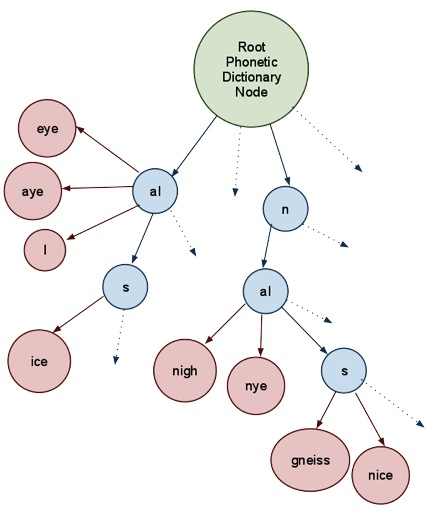
\includegraphics[width=90mm]{wordTree.jpg}
\captionfonts
\caption[Word Tree]{Word tree}
\label{fig:wordTree}
\end{figure}

We can use this dictionary tree method to discover all valid orthographic interpretations for any phonetic sequence of our root orthographic phrase, as shown in figure~\ref{fig:aNiceColdHourPhoneToOrthoGraph} for the phrase ``a nice cold hour''.


\begin{figure}[h]
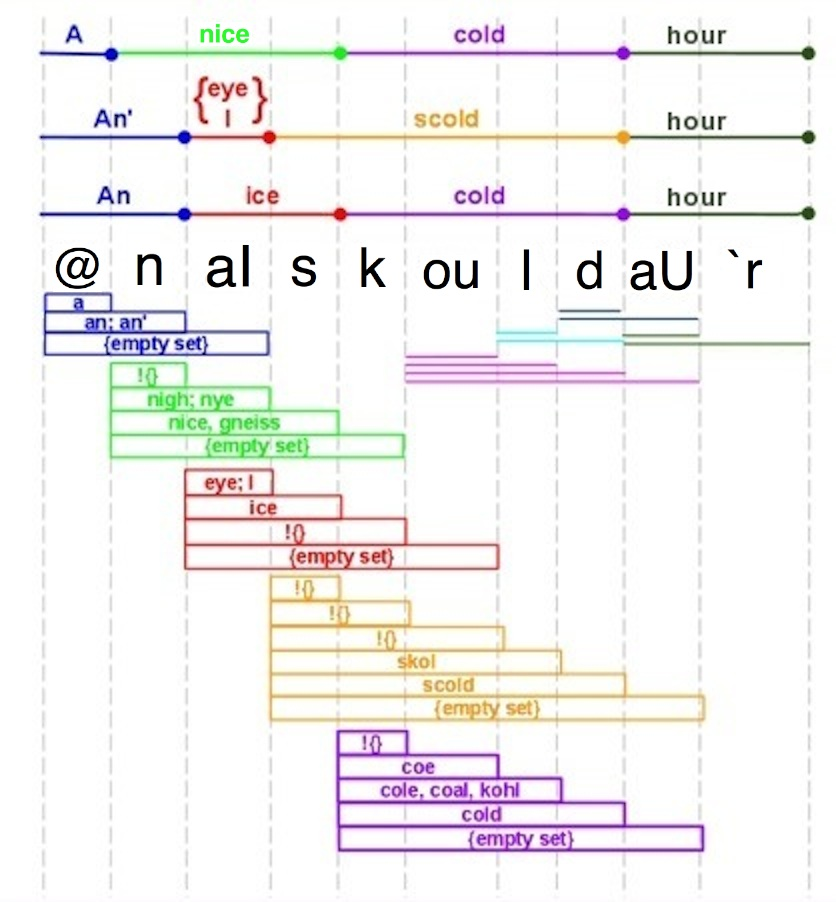
\includegraphics[width=\textwidth]{aNiceColdHourPhoneToOrthoBreakdown.jpg}
\captionfonts
\caption[Phoneme to ortho graph of ``a nice cold hour'']{Phoneme to ortho graph of ``a nice cold hour''}
\label{fig:aNiceColdHourPhoneToOrthoGraph}
\end{figure}

Once we have grabbed all the orthographic interpretations for each phonetic sequence, we combine them all into an orthographic oronym phrase list. This process may leave us with some redundant oronyms, so we de-duplicate that list.

After this, we have a list of all unique and valid oronyms for the original root phrase.

In the case of ``a nice cold hour", this returns 290 oronyms, as seen in the first column of figure~\ref{table:aNiceColdHourOronymWithFreqsTable}.



The pseudocode for this process can be reviewed in figure~\ref{fig:psuedoCode:discoverOronymsForPhrase}.





\subsection{Word Frequency Evaluation}
\label{subsection:wordFrequencyEvaluation}

Next, we want to evaluate all our oronyms based on how common each oronym's component words are.  For example, ``a nice cold hour" is much more likely to be heard ``a gneiss cold hour," even though both are phonetically identical.

To do this, we tokenize each oronym phrase into its component words, once again delimiting by non-newline whitespaces. 

Then, we query our phonetic dictionary with each word to get that word's frequency value.  We store each word's value separately. When we have retrieved the frequencies for all the words in a phrase, we then sum up all the frequencies  to give a combined frequency of the entire phrase.

You can see these frequency counts for each word in all oronyms of the phrase ``a nice cold hour" in table ~\ref{table:aNiceColdHourOronymWithFreqsTable}.




\section{Visual Representation}
\label{section:implementation:visualRepresentation}

We created two different oronym visualizations. The first, oronym trees, were chosen for their ability to show the phonetic dead ends that may happen during oronym generation. Our particular oronym tree visualization is written in C++ using OpenGL, which allows for future integration into another codebase. 

The second visualization shows all valid oronyms of a root phrase using what is known as a sunburst diagram. These sunburst diagrams were created using the ProtoVis library, and use javascript data files with html wrappers. The javascript data files were generated using the same C++ code that the first visualization used, so both visualizations show similar data.  However, the oronym sunburst diagrams more easily exhibit the weighting of the different oronym paths with their frequency dictionary values.


\subsection{Oronym Tree Visualization}
\label{subsection:oronymTreeVisualization}

We go about building the visual representation of the oronym parse tree in much the same way that we build the textual list of oronyms, with one important caveat: our oronym parse trees may contain oronym fragments.   To deal with these, we've got to keep track of all our abandoned sub-phrases. For example, for the root oronym phrase ``iced ink'' (\texttt{aI s t I N k}), a listener may hear and interpret up to ``I sting''(\texttt{aI s t I N)}, and then be confused when the last phone, \texttt{k}, comes along.

\begin{wrapfigure}{r}{0.5\textwidth}
\begin{center}
\begin{tabular}{|l|}
\hline
aye sting xxx \\
aye stink \_\_\_SUCCESS!\_\_\_ \\
ay sting xxx \\
ay stink \_\_\_SUCCESS!\_\_\_ \\
eye sting xxx \\
eye stink  \_\_\_SUCCESS!\_\_\_ \\
i sting xxx \\
i stink \_\_\_SUCCESS!\_\_\_ \\
ice ting xxx \\
ice xxx \\
iced ink \_\_\_SUCCESS!\_\_\_ \\
\hline
\end{tabular}
\captionfonts
\caption[IcedInkOronymsWithPartials]{All partial and complete oronyms for the phrase ``iced ink''}
\label{fig:oronymTree:IcedInkOronyms}
\end{center}
\end{wrapfigure}

Our algorithm for building the tree diagram is recursive, called from a parent function that draws the tree's `seed' sphere. This parent function engages in a depth-first traversal of the oronym tree, and is documented in figure ~\ref{fig:psuedoCode:buildAndDrawFullTree}


We start in the parent function by getting all the oronyms of our orthographic phrase, using the process outlined in sections  ~\ref{subsection:stepOneFindAllSAMPAphrase} and ~\ref{subsection:stepTwoFindOrthoforSAMPA}.  However, instead of ignoring any incomplete orthographic interpretation of a phonetic sequence, as we do in section~\ref{subsection:stepTwoFindOrthoforSAMPA}, we add the incomplete phrases to the list of oronyms, keeping track of them by appending `xxx' or `fff' to the end of each incomplete oronym string. For example, as shown in figure ~\ref{fig:oronymTree:IcedInkOronyms}. the phrase ``iced ink'' may only have has five complete oronyms, but it has six additional oronym fragments, making for 11 possible interpretations.   


Then, we tokenize our phrases by whitespace, and look up the frequency of each word, as shown for ``iced ink'' in figure ~\ref{fig:oronymTree:FreqValsForIcedInkOronyms}.  We will later scale our branches' radii using the maximum and minimum word frequency values found during this run. In this case, the maximum is 9,937,877 for the word ``I'', and the minimum is 124 for the word ``ting''.

\begin{figure}[ht]
\begin{center}
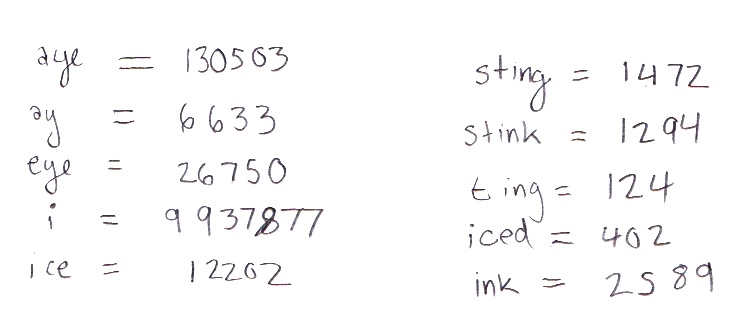
\includegraphics[width=.5\textwidth]{Fig3_3_2_FreqValsForIcedInkOronyms.jpg}
\captionfonts
\caption[FreqValsForIcedInkOronyms]{Frequency values for all unique words in ``iced ink'' oronyms}
\label{fig:oronymTree:FreqValsForIcedInkOronyms}
\end{center}
\end{figure}

Once we have all partial and complete oronyms, plus the maximum and minimum word frequency values found in all those phrases, we pass them into our recursive function, along with the radius of the seed sphere.  That radius will be the beginning radius of each root-level branch, as shown in figure ~\ref{fig:oronymTree:seedSphere}

\begin{figure}[ht]
\begin{center}
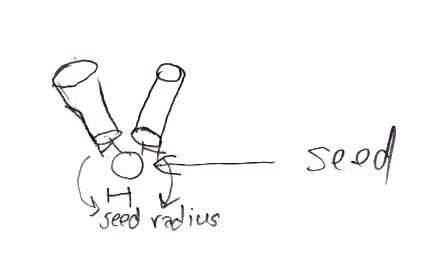
\includegraphics[width=.33\textwidth]{Fig3_3_3_SeedSphere.jpg}
\captionfonts
\caption[Seed Sphere vs branch radius comparison]{Seed Sphere vs branch radius comparison}
\label{fig:oronymTree:seedSphere}
\end{center}
\end{figure}

Inside our recursive function, we pull the first word out of each orthographic phrase, and create a set of unique first words, as seen in figure ~\ref{fig:oronymTree:grabFirstWordsIcedInkOronyms}.  

\begin{figure}[ht]
\begin{center}
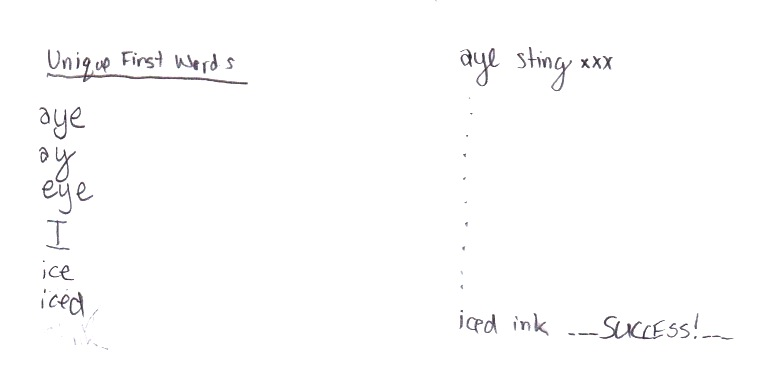
\includegraphics[width=.5\textwidth]{Fig3_3_4_GrabFirstWordsIcedInkOronyms.jpg}
\captionfonts
\caption[Unique first words of Iced Ink oronyms]{All uniqueirst words of ``iced ink'' oronyms}
\label{fig:oronymTree:grabFirstWordsIcedInkOronyms}
\end{center}
\end{figure}

We then go through this set of unique first words iteratively.

For each word, we look up frequency in the phonetic dictionary.  Then, we use the maximum and minimum frequencies that we found in our parent function, plus constants for maximum and minimum radius size, to scale that frequency into a usable radius size. 

Then, we check the contents of the word string. 

If the word is ``xxx'' or ``fff'', then it's not a word at all---just an indication of the dead end of an oronym fragment.  In this case, as seen in figure ~\ref{fig:oronymTree:deadEndIceTing}, we draw a red sphere with the radius of the branch's ancestor, using the radius parameter passed into our recursive function for `lastRadius'.  

\begin{figure}[ht]
\begin{center}
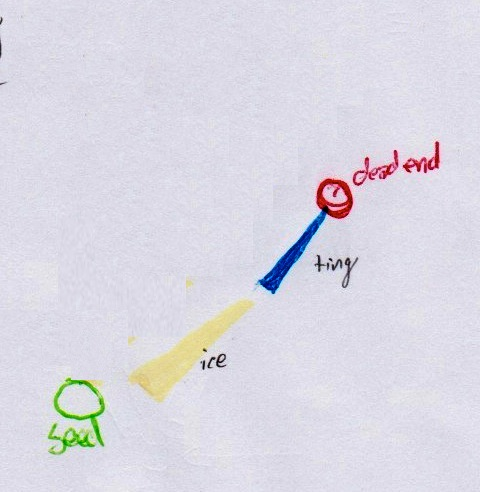
\includegraphics[width=.33\textwidth]{Fig3_3_5_DeadEndIceTing.jpg}
\captionfonts
\caption[Dead end for oronym fragment Ice Ting]{Dead end sphere for oronym fragment ``ice ting''}
\label{fig:oronymTree:deadEndIceTing}
\end{center}
\end{figure}

If the word is ``\_\_\_SUCCESS!\_\_\_'', that indicates a full oronym has been successfully found, and is terminating at that point. This time, we draw a green sphere using the \emph{lastRadius} parameter for size, as seen in figure ~\ref{fig:oronymTree:IStink} for the phrase ``I stink''.

\begin{figure}[ht]
\begin{center}
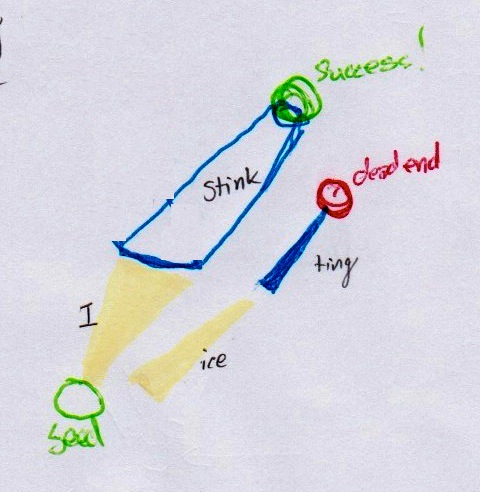
\includegraphics[width=.33\textwidth]{Fig3_3_6_IStink.jpg}
\captionfonts
\caption[Success indicator sphrere for complete oronym]{Success indicator sphrere for complete oronym ``I stink''}
\label{fig:oronymTree:IStink}
\end{center}
\end{figure}

If the word isn't ``xxx'', ``fff'', or ``\_\_\_SUCCESS!\_\_\_'', it is a valid orthographic word, and we draw a cylinder ``branch'' representing that word. The cylinder's bottom radius is equal to \emph{lastRadius}, and the top radius is equal to the scaled radius that we derived using the word's frequency.  An example of this branch radius scaling is show in figure ~\ref{fig:oronymTree:CylinderRadiusDiff}.

\begin{figure}[ht]
\begin{center}
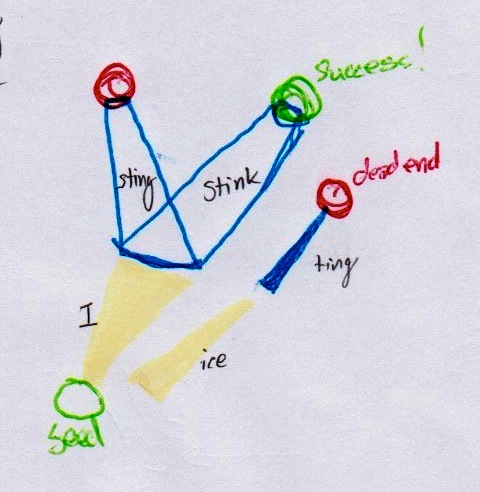
\includegraphics[width=.33\textwidth]{Fig3_3_7_CylinderRadiusDiff.jpg}
\captionfonts
\caption[Branch radius scaling to show frequency differences]{Scaled branch radii showing frequency difference}
\label{fig:oronymTree:CylinderRadiusDiff}
\end{center}
\end{figure}

After we draw the cylinder, we then go through the full list of phrases, and compile a list of all phrases that start with the word we just drew the cylinder for, as in figure ~\ref{fig:oronymTree:PhrasesStartingWithAye}.  Then, we remove the first word from each of those phrases, deduplicating the resulting list of ``tail'' phrases, which is shown in figure ~\ref{fig:oronymTree:TailPhrasesForAye}.

\begin{figure}[ht]
\begin{center}
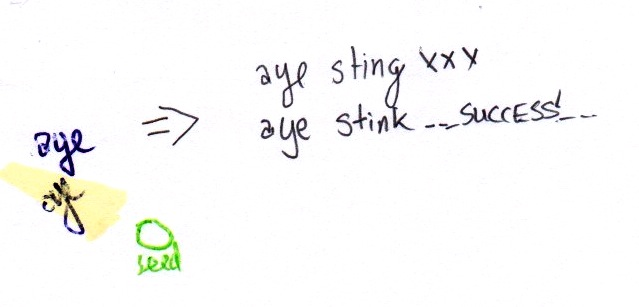
\includegraphics[width=.5\textwidth]{Fig3_3_8_PhrasesStartingWithAye.jpg}
\captionfonts
\caption[Oronym Phrases starting with aye]{All oronym phrases of ``iced ink'' starting with ``aye''}
\label{fig:oronymTree:PhrasesStartingWithAye}
\end{center}
\end{figure}

\begin{figure}[ht]
\begin{center}
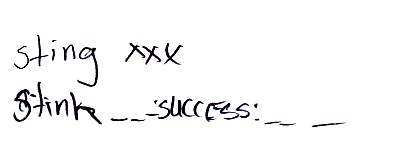
\includegraphics[width=.5\textwidth]{Fig3_3_9_TailPhrasesForAye.jpg}
\captionfonts
\caption[Tail Phrases for aye]{Tail phrases for oronyms of ``iced ink'' that begin with ``aye''}
\label{fig:oronymTree:TailPhrasesForAye}
\end{center}
\end{figure}

Then, we change our material color (so that different levels of branches will be different colors), and make a recursive call to our current function, passing as parameters the scaled radius and the list of tail phrases.

After this recursive call, we change our color material back to whatever it was before the call, and then continue on to the next unique first word in our set, which, in this case, is ``ay.''

Once we have looped through all our unique first words, we know we're done drawing that set of branches, and we return.  

This gives us the oronym parse tree seen in figure ~\ref{fig:oronymTree:treeIcedInk}.  As shown in figure ~\ref{fig:oronymTree:treeIcedInkAnnotated} (the annotated version of figure ~\ref{fig:oronymTree:treeIcedInk}) each branch on the tree represents a single orthographic word.

\begin{figure}[ht]
\begin{center}
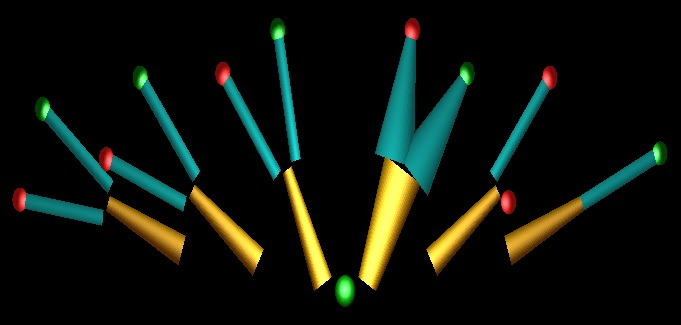
\includegraphics[width=.5\textwidth]{OronymTree_blackbg_IcedInk.jpg}
\captionfonts
\caption[Oronym tree for the phrase iced ink]{Oronym tree for the phrase ``iced ink''}
\label{fig:oronymTree:treeIcedInk}
\end{center}
\end{figure}


\begin{figure}[ht]
\begin{center}
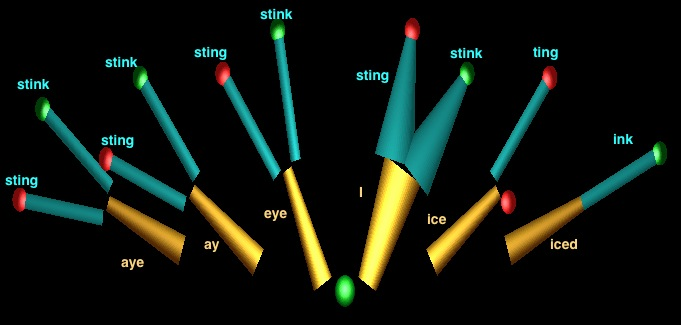
\includegraphics[width=\textwidth]{OronymTree_blackbg_IcedInk_annotated.jpg}
\captionfonts
\caption[Annotated oronym tree for the phrase iced ink]{Annotated oronym tree for the phrase ``iced ink''}
\label{fig:oronymTree:treeIcedInkAnnotated}
\end{center}
\end{figure}






%\begin{figure}
%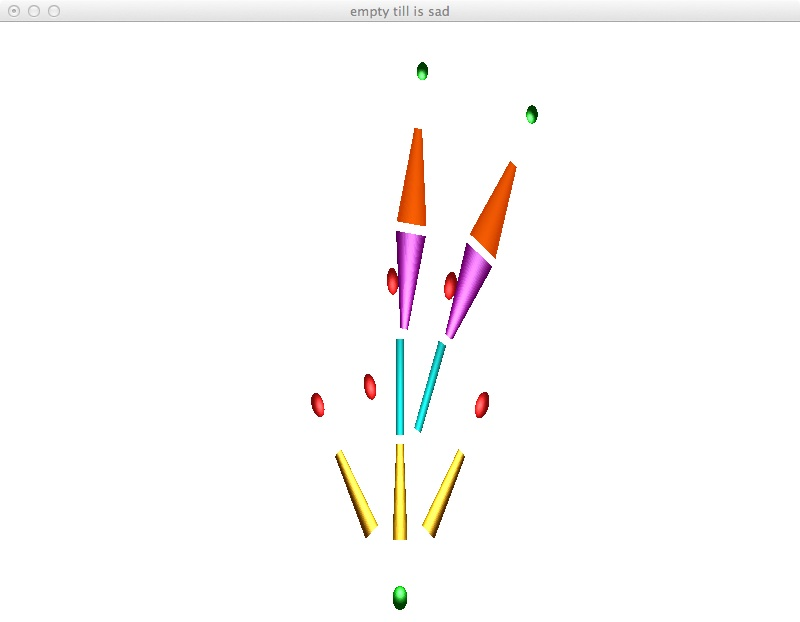
\includegraphics[width=150mm]{emptyTillIsSad.jpg}
%\captionfonts
%\caption[Oronym Parse Tree]{ This is the parse tree for the phrase ``empty till is sad" }
%\label{fig:treeEmptyTillIsSad}
%\end{figure}

%\begin{figure}
%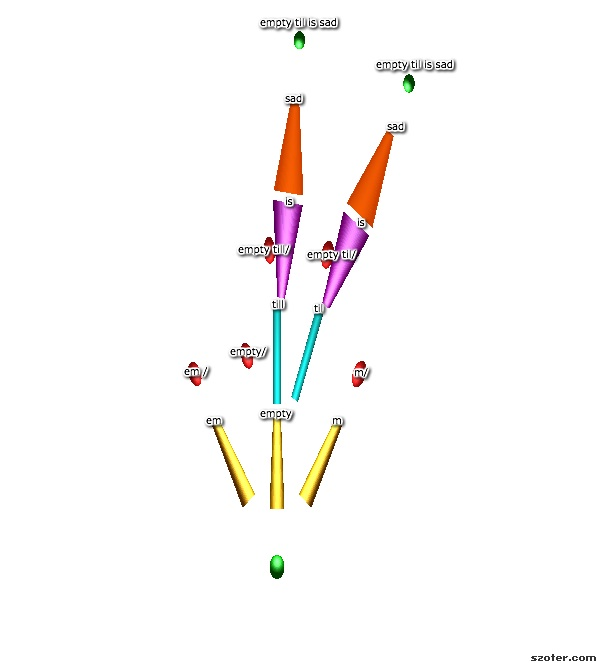
\includegraphics[width=150mm]{emptyTillIsSadAnnotated.jpg}
%\captionfonts
%\caption[Annotated Oronym Parse Tree]{ This is the annotated parse tree for the phrase ``empty till is sad" }
%\label{fig:treeEmptyTillIsSadAnnotated}
%\end{figure}



\subsection{Oronym Sunburst Visualization}
\label{subsection:oronymSunburstVisualization}

For our second visualization type, we chose to use sunburst diagrams.  


\subsubsection{Sunburst diagram generation}
\label{subsection:oronymsunburst:sunburstDiagramGeneration}


To generate these sunburst diagrams, we modified our existing C++ program to output data in the Protovis.js format, which is seen in figure ~\ref{fig:oronymsunburst:exampleSunburstJS}. 

\begin{figure}
\begin{tabbing}
var \textcolor{RoyalBlue}{root} = \{\= \\
\>  \textcolor{Red}{Child1}: \{\= \\
\>\>    \textcolor{Green}{Child1A}: \{\= \\
\>\>\>      \textcolor{Violet}{Child1Ai}: \textcolor{VioletRed}{actualCount}, \\
\>\>\>      \textcolor{Violet}{Child1Aii}: \textcolor{VioletRed}{actualCount} \\
\>\>    \}, \\
\>\>    \textcolor{Green}{Child1B}: \{ \\
\>\>\>      \textcolor{Violet}{Child1Bi}: \textcolor{VioletRed}{actualCount} \\
\>\>    \} \\
\>  \},  \\
\>  \textcolor{Red}{Child2}: \{ \\
\>\>    \textcolor{Green}{Child2A}: \{ \\
\>\>\>      \textcolor{Violet}{Child2Ai}: \textcolor{VioletRed}{actualCount}, \\
\>\>\>      \textcolor{Violet}{Child2Aii}: \textcolor{VioletRed}{actualCount} \\
\>\>    \} \\
\>  \} \\
\};
\end{tabbing}
\captionfonts
\caption[Example Sunburst Diagram]{ Protovis sunburst data format: This example sunburst data file, once the \emph{actualCount} occurances were replaced with actual values, would generate a sunburst diagram}
\label{fig:oronymsunburst:exampleSunburstJS}
\end{figure}


\begin{figure}
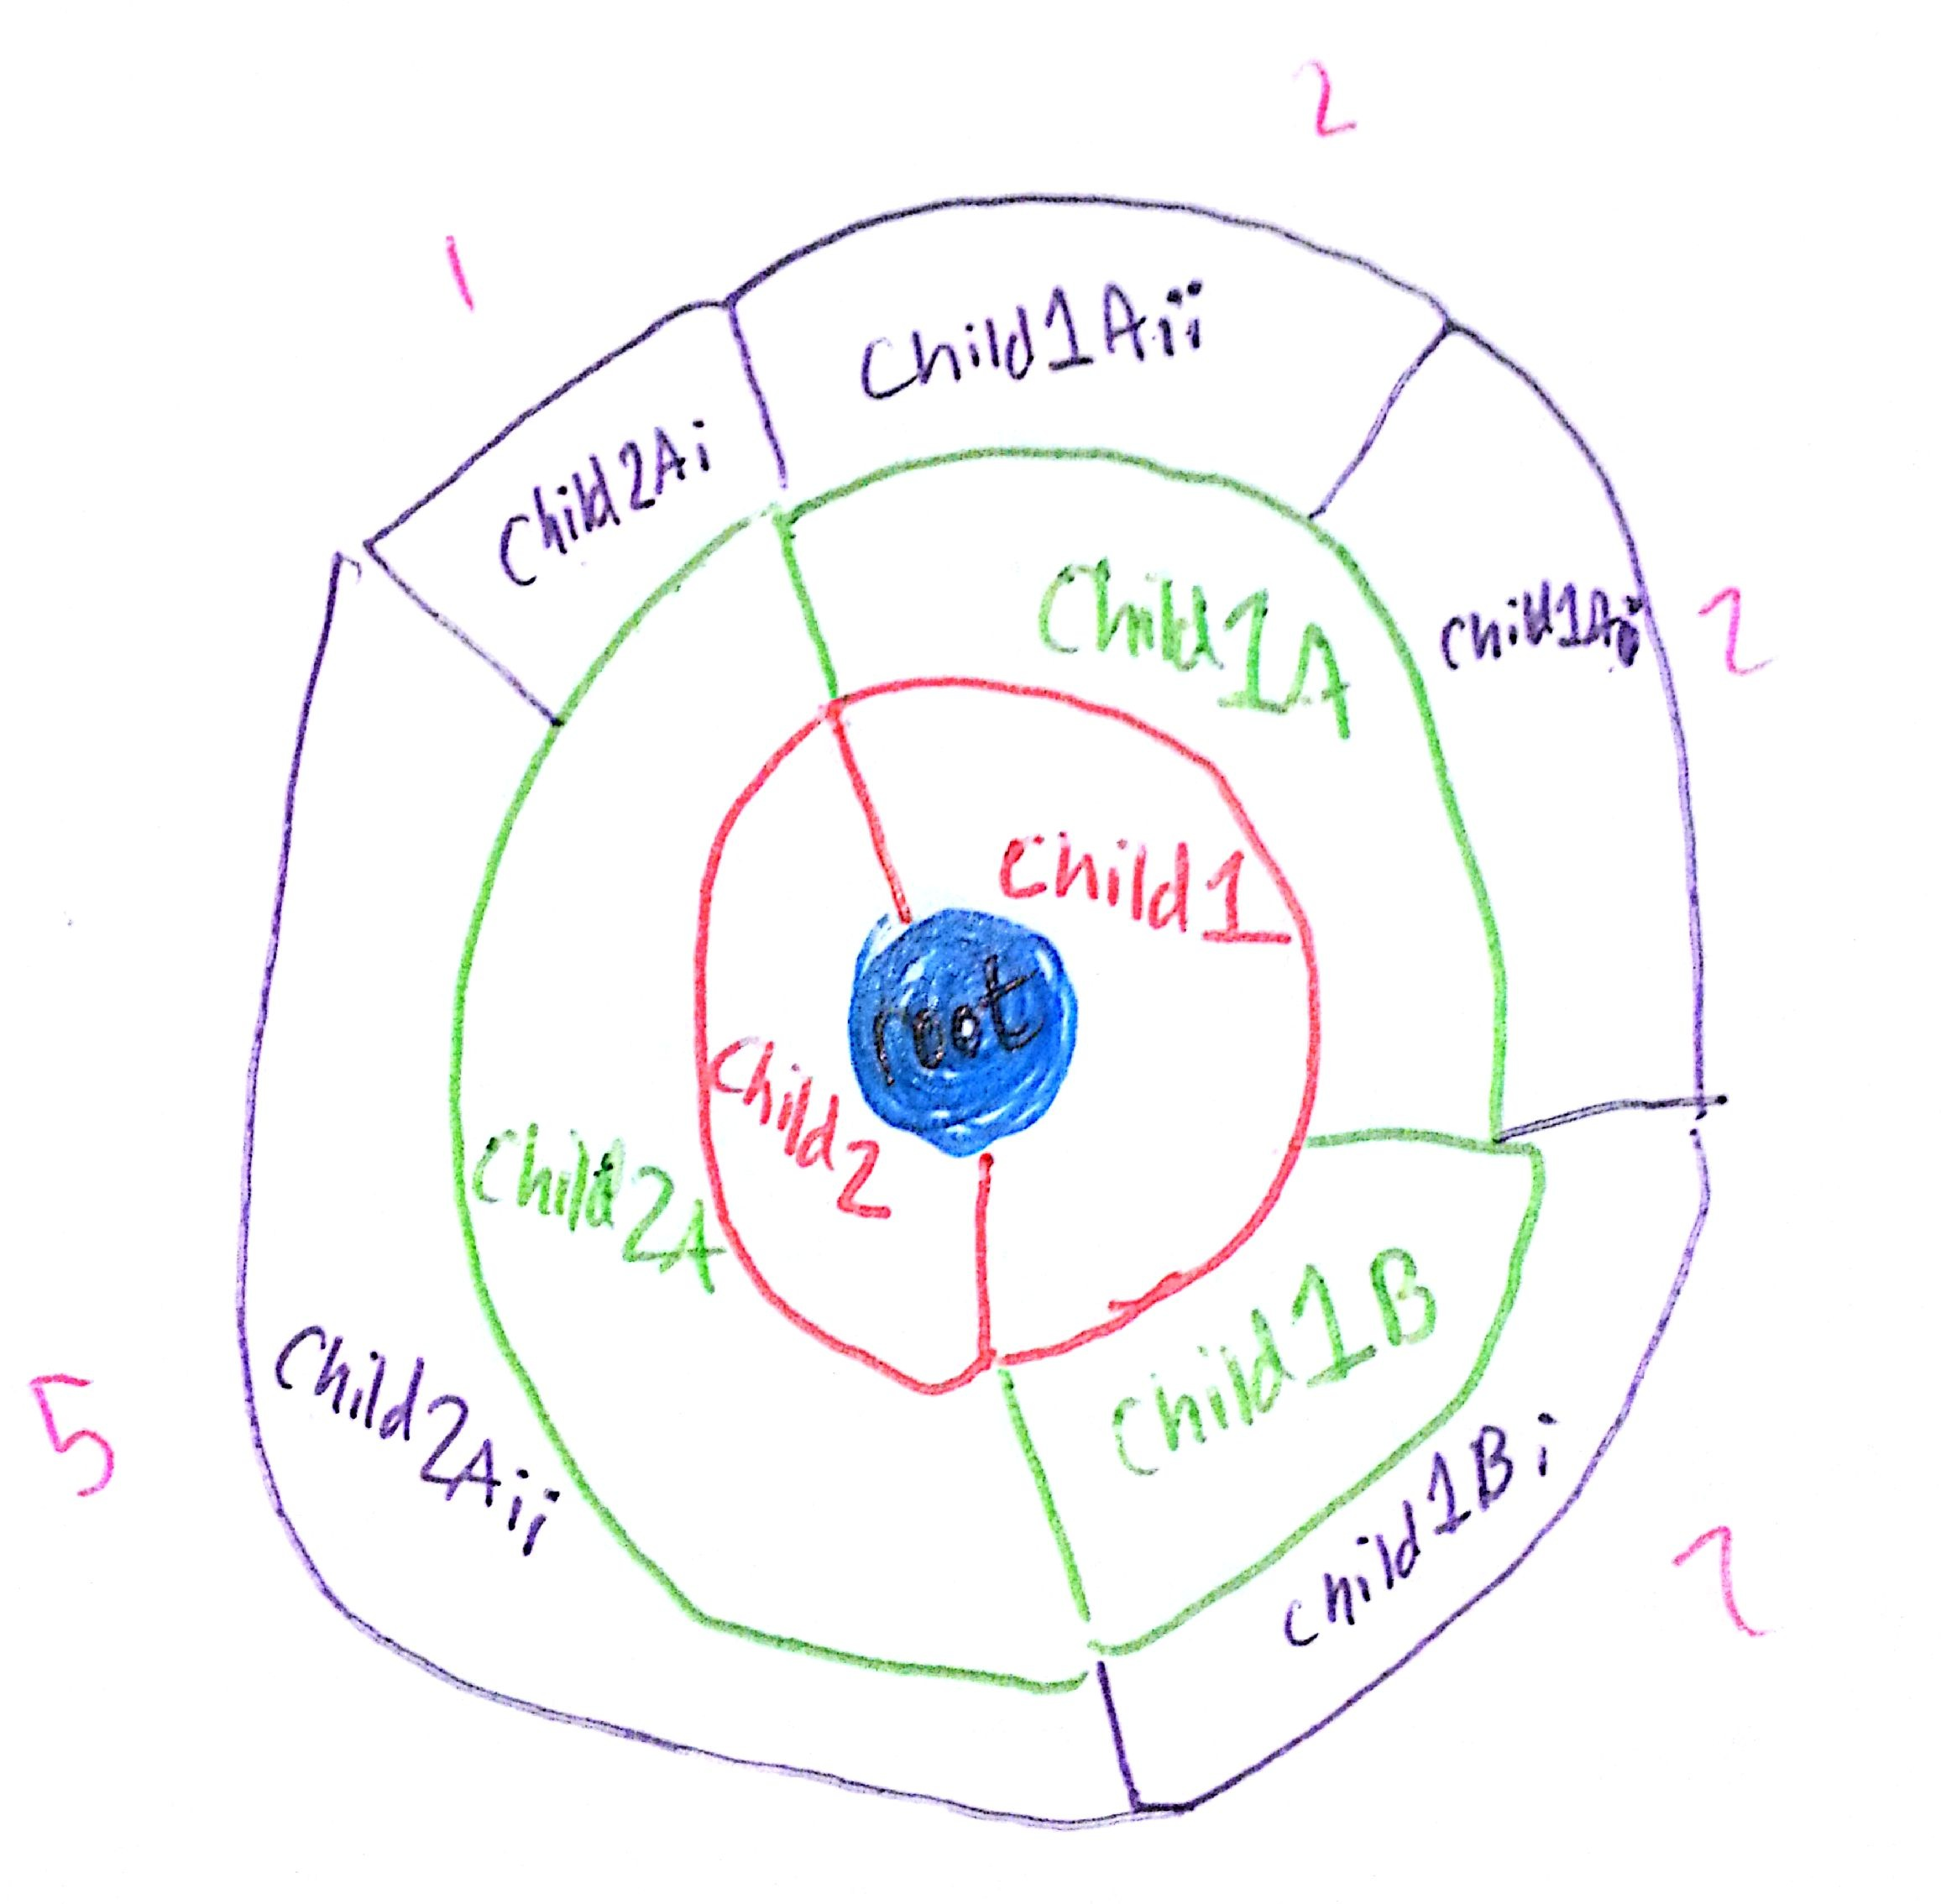
\includegraphics[width=150mm]{SunburstExampleDiagramRough.jpg}
\captionfonts
\caption[Example Sunburst Diagram]{ This example sunburst diagram is what would be generated by the example data file in figure ~\ref{fig:oronymsunburst:exampleSunburstJS} }
\label{fig:oronymSunburst:exampleSunburst}
\end{figure}


The labels before the colons are displayed on the diagram in their respective segment, as seen in figure ~\ref{fig:oronymSunburst:exampleSunburst}. 

Some minor adjustments were made to the C++ output. The Protovis document format does not allow for non-alphanumeric characters to appear in labels, so words like ``ice-cold'' or ``it's'' caused errors. We found it necessary to remove all non-alphanumeric characters so that the sunbursts would generate successfully. 

One of the main benefits of the Protovis data format is that, once the relevant data has been formatted correctly, many different types of graphs can be trivially generated. For our data format, we can generateboth sunburst and icicle graph views.  We chose to use sunburst graphs, as results from an informal user poll indicated a preference for sunbursts over icicles.

\subsubsection{Reading a sunburst diagram}
\label{subsection:oronymsunburst:readingASunburstDiagram}

To read a sunburst diagram, start at the very center, which in our case is labelled ``root''. Then, pick any one segment from the first ring surrounding the root. The word contained in this segment will be the first word in the oronym phrase.

Next, look at all the outer arc segments that directly touch the first segment picked. Every word in those adjoining arc segments is a valid subsequent word for the oronym phrase starting with the word in the first, inner arc segment.

Continue this process, using one segment per level, until you reach a segment that has no subsequent outer segments. At this point, you will have compiled a full oronym phrase. The size of the final outer segment, relative to size of the rest of the segments in its particular ring, shows you the relative commonness of the phrase whose path ends at that segment.

So, for example, interpreting the sunburst diagram in figure ~\ref{fig:oronymSunburst:exampleSunburst} would result in the following faux-oronym phrases: ``child1 child1A child1Ai'', ``child1 child1A child1Aii'', ``child1 child1B child1Bi'', ``child2 child2A child2Ai'', and finally, ``child2 child2A child2Aii''.

\subsubsection{Example Sunburst Diagrams}
\label{subsection:oronymsunburst:exampleSunburstDiagrams}

We generated several types of sunburst diagrams, using both artificially-balanced path weights and using the frequency values for each path derived from our UNISYN dictionary.  A clearer view of how we used sunburst diagrams can be provided with some concrete examples. 

Consider the two sunburst diagrams for the oronyms of the phrase ``iced ink'', shown in figures ~\ref{fig:oronymsunburst:iStinkEqualWeight} and ~\ref{fig:oronymsunburst:iStinkUNISYNWeight}. The phrase ``iced ink'' has five different oronyms: ``iced ink'', ``ay stink'', ``aye stink'', ``eye stink'', and ``I stink''. The five different outer segments (which are easier to see on the equal-weighted sunburst diagram in figure ~\ref{fig:oronymsunburst:iStinkEqualWeight}) represent the end word of each of those oronyms. The sunburst diagram that uses the frequency metric (shown in figure ~\ref{fig:oronymsunburst:iStinkUNISYNWeight}) shows that people are overwhelmingly more likely to hear ``I stink'' than any other possible oronym.

\begin{figure}
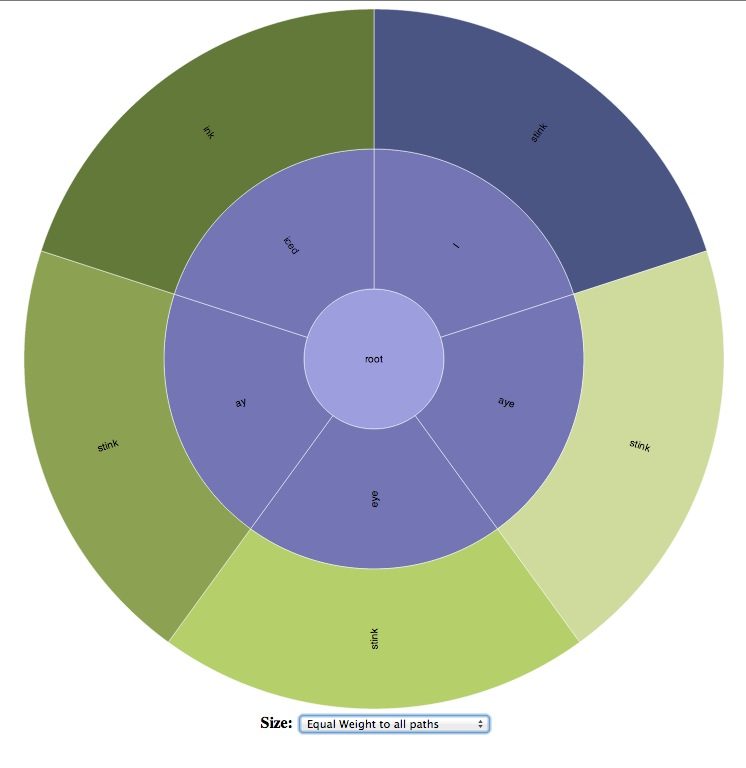
\includegraphics[width=150mm]{iStink_EqualWeight.jpg}
\captionfonts
\caption[Equally-Weighted Sunburst Diagram for the oronyms of ``iced ink'']{Equally-Weighted Sunburst Diagram for the oronyms of ``iced ink''}
\label{fig:oronymsunburst:iStinkEqualWeight}
\end{figure}


\begin{figure}
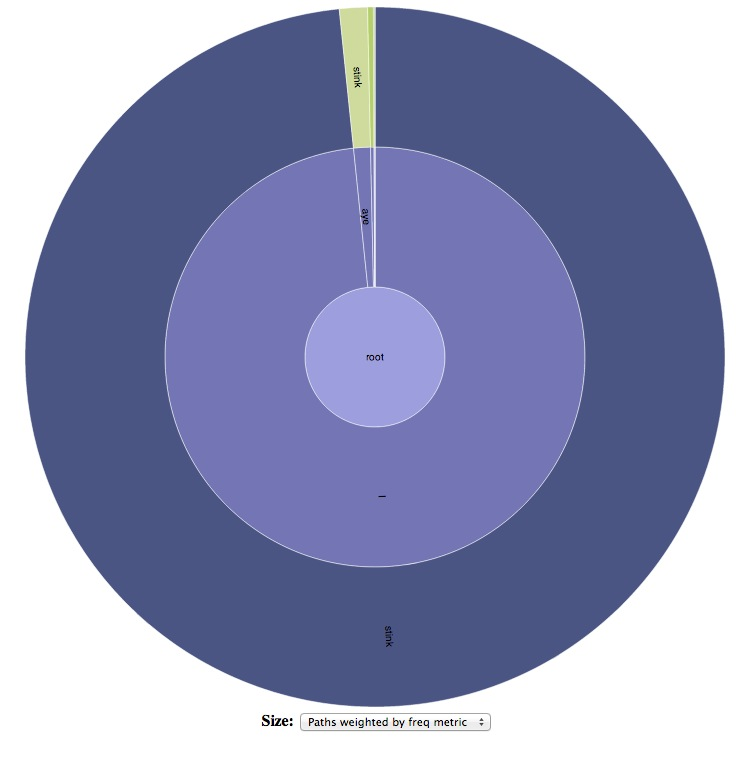
\includegraphics[width=150mm]{iStink_Weighted.jpg}
\captionfonts
\caption[Sunburst Diagram for the oronyms of ``iced ink'' weighted by UNISYN freq metric]{Sunburst Diagram for the oronyms of ``iced ink'' weighted by UNISYN freq metric }
\label{fig:oronymsunburst:iStinkUNISYNWeight}
\end{figure}

For a more complicated example, take the sunburst diagrams for oronyms of the phrase ``why that's insane''. The diagram shown in figure ~\ref{fig:oronymsunburst:whyThatsInsaneEqualWeight} shows the seven possible oronyms that can result from phonetic interpretation of that phrase, and even though one phrase is one word shorter than all the rest, the weights of the paths remain equal. The weighted diagram, shown in figure ~\ref{fig:oronymsunburst:whyThatsInsaneUNISYNWeight}, shows that the UNISYN-predicted frequency of each phrase's occurance. 


\begin{figure}
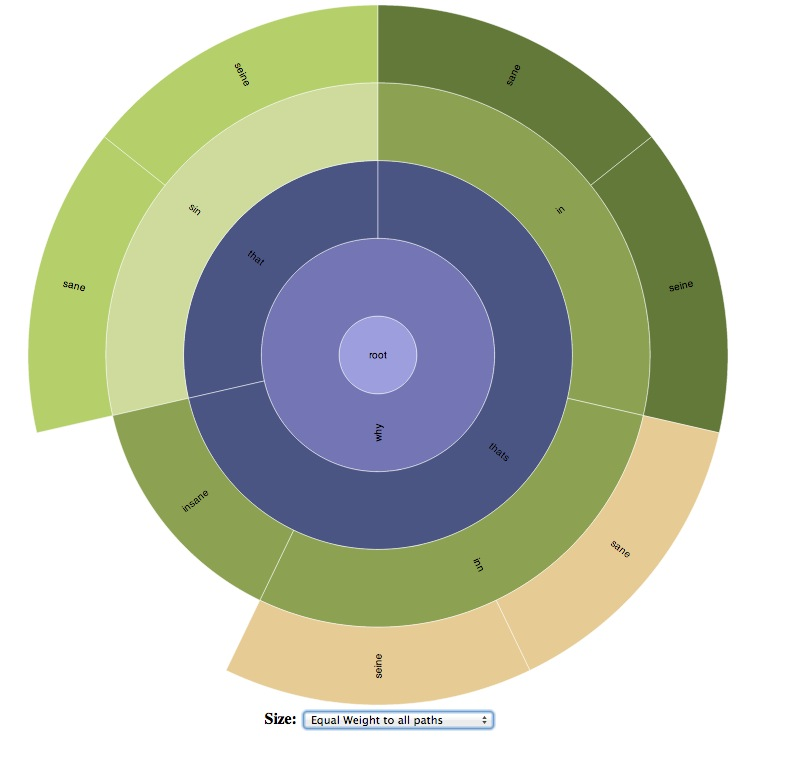
\includegraphics[width=150mm]{whyThatsInsane_EqualWeight.jpg}
\captionfonts
\caption[Equally-Weighted Sunburst Diagram for the oronyms of ``why that's insane'']{Equally-Weighted Sunburst Diagram for the oronyms of ``why that's insane''}
\label{fig:oronymsunburst:whyThatsInsaneEqualWeight}
\end{figure}


\begin{figure}
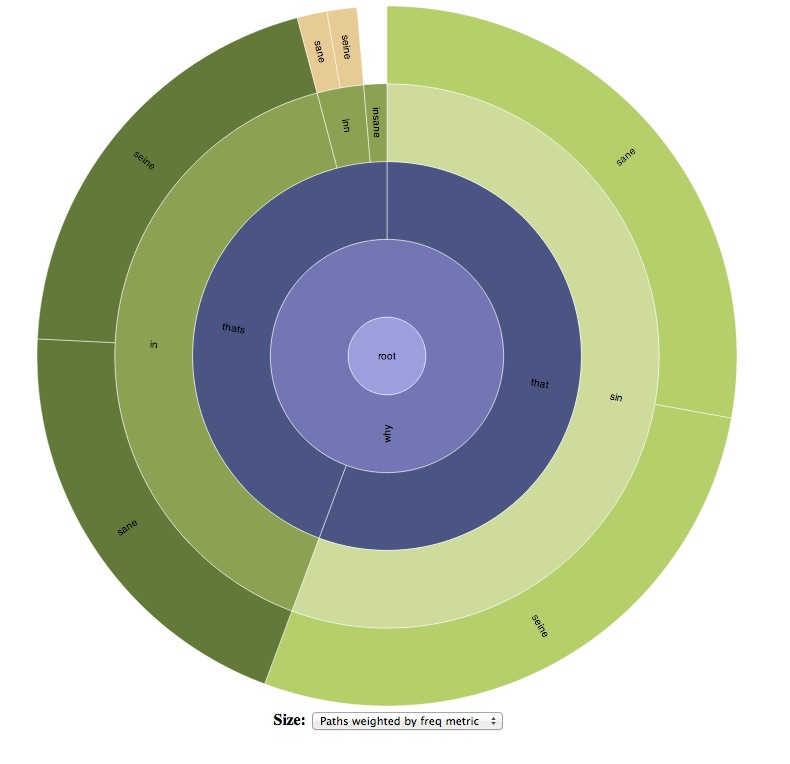
\includegraphics[width=150mm]{whyThatsInsane_UNISYN.jpg}
\captionfonts
\caption[Sunburst Diagram for the oronyms of ``why that's insane'' weighted by UNISYN freq metric]{Sunburst Diagram for the oronyms of ``why that's insane'' weighted by UNISYN freq metric }
\label{fig:oronymsunburst:whyThatsInsaneUNISYNWeight}
\end{figure}


Lastly, consider the sunburst diagrams for the phrase we chose to focus on in our user study: ``an ice cold hour''.  As seen in figure ~\ref{fig:oronymsunburst:anicecoldhourEqualWeight}, the equally-weighted sunburst diagram shows all possible oronym paths. When compared to the sunburst diagram in figure ~\ref{fig:oronymsunburst:anicecoldhourUNISYNWeight} that uses the UNISYN-derived frequency metric, we can see that some paths, such as those that begin with the word ``a'', are much more likely to be heard than those that begin, for example, with the word ``n''. 


\begin{figure}
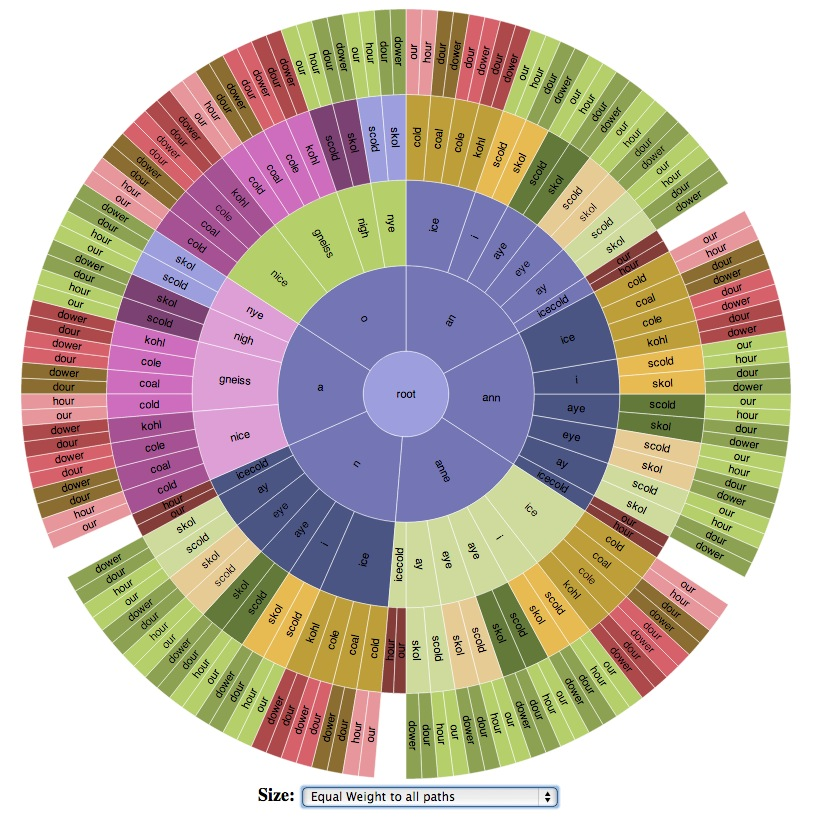
\includegraphics[width=150mm]{aNiceColdHour_UNISYN_FreqMetric_EqualWeight.jpg}
\captionfonts
\caption[Equally-Weighted Sunburst Diagram for the oronyms of ``an ice cold hour'']{Equally-Weighted Sunburst Diagram for the oronyms of ``an ice cold hour''}
\label{fig:oronymsunburst:anicecoldhourEqualWeight}
\end{figure}


\begin{figure}
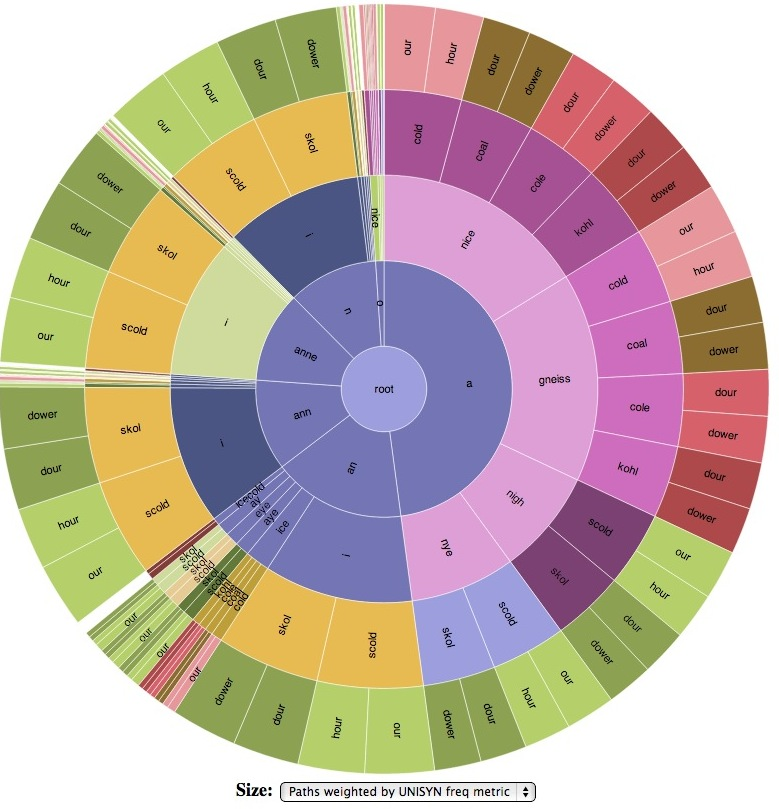
\includegraphics[width=150mm]{aNiceColdHour_UNISYN_FreqMetric.jpg}
\captionfonts
\caption[Sunburst Diagram for the oronyms of ``an ice cold hour'' weighted by UNISYN freq metric]{Sunburst Diagram for the oronyms of ``an ice cold hour'' weighted by UNISYN freq metric }
\label{fig:oronymsunburst:anicecoldhourUNISYNWeight}
\end{figure}


